\chapter{Introducción a matplotlib\\ Introduction to matplotlib}
\begin{paracol}{2}
    Visualizar los datos es fundamental para poder comprender y transmitir ideas e información en ciencias e ingeniería.
    Python tiene numerosas funciones gráficas que para mostrar muchos tipos de gráficos. Una de las librerías para visualizar datos de uso más extendido es \href{https://matplotlib.org/stable/}{matplotlib} a la que dedicamos este capítulo.
    \switchcolumn
    Visualising data is essential for understanding and conveying ideas and information in science and engineering.
    Python has numerous graphics functions for displaying many types of graphics. One of the most widely used data visualisation libraries is \href{https://matplotlib.org/stable/}{matplotlib} to which we dedicate this chapter.
    \switchcolumn
    Importaremos la biblioteca matplotlib de la siguiente manera
    \switchcolumn
    We can import matplotlib as follows:
\end{paracol}

\begin{minted}{python}
    import matplotlib as mpl
\end{minted}
\begin{paracol}{2}
    \paragraph{matplotlib.pyplot} es una colección de funciones que hacen que matplotlib funcione como MATLAB. Cada función de pyplot realiza algún cambio en una figura: por ejemplo, crea una figura, crea un área de trazado en una figura, traza algunas líneas en un área de trazado, decora el trazado con etiquetas, etc.

    En matplotlib.pyplot la figura se conserva a través de las llamadas a funciones, de modo que las funciones de trazado se ejecutan sobre los ejes actuales.
    \switchcolumn
        \paragraph{matplotlib.pyplot} is a collection of functions that make matplotlib work like MATLAB. Each pyplot function makes some change to a figure: for example, it creates a figure, creates a plot area in a figure, draws some lines in a plot area, decorates the plot with labels, etc.

        In matplotlib.pyplot the figure is preserved across function calls, so that the plotting functions are executed on the current axes.
\switchcolumn
Para crear gráficas usando Matplotlib necesitaremos una figura. Cada figura tiene un par (o más) de ejes y un área que es donde se dibujarán los puntos en el sistema de coordenadas que decidamos. Además podremos poner títulos, leyendas etc...

\switchcolumn

To create graphs using Matplotlib we will need a figure. Each figure has a pair (or more) of axes and an area which is where the points will be drawn in the coordinate system of your choice. In addition we can put titles, legends etc...

\switchcolumn

La manera más sencilla de crear una figura es empleando el método \texttt{figure} que creará una figura en la que posteriormente podremos añadir ejes, títulos y más cosas. Simplemente llamando a \texttt{figure} creamos un objeto de tipo figura, aunque también podemos darle de manera opcional parámetros como el tamaño, el color de fondo y más.

\switchcolumn
The easiest way to create a figure is to use the \texttt{figure} method which will create a figure to which we can later add axes, titles and more. Simply by calling \texttt{figure} we create an object of type figure, although we can also optionally give it parameters such as size, background colour and more.
\end{paracol}

\begin{paracol}{2}

\end{paracol}
\begin{minted}{python}
import matplotlib.pyplot as plt
fig = plt.figure(figsize=(2, 2), facecolor='lightskyblue',
                 layout='constrained')
fig =plt.figure            
\end{minted}

\section{Dibujar en 2D}
\begin{paracol}{2}
    La manera más sencilla de dibujar usando matplotlib.pyplot es mediante el método \texttt{plot}. A este método le pasaremos dos vectores con las coordenadas $x$ e $y$ de los puntos que queremos representar (evidentemente tendremos que asegurarnos de que tienen la misma longitud).

    Por ejemplo si generamos unos vectores de coordenadas como los siguientes $x=(0,2,-1,-2)$ e $y=(0,3,2,-4)$, y se los pasamos al método \texttt{plot} pyplot dibujará los puntos $(x,y)$ y los unirá con rectas, como puede verse en la figura \ref{fig:pyplot-simple}.
    \switchcolumn
        The easiest way to draw using matplotlib.pyplot is by using the \texttt{plot} method. To this method we will pass two vectors with the $x$ and $y$ coordinates of the points we want to represent (obviously we will have to make sure that they have the same length).  

            For example, if we generate coordinate vectors such as $x=(0,2,-1,-2)$ and $y=(0,3,2,-4)$, and pass them to the pyplot method, it will draw the points $(x,y)$ and join them with straight lines, as can be seen in the figure \ref{fig:pyplot-simple}.
        
\end{paracol}
\begin{minted}{python}
import numpy as np
import matplotlib.pyplot as plt

x=np.array([0, 2, -1, -2])
y=np.array([0, 3, 2, -4])
plt.figure
plt.plot(x,y)
\end{minted}
\begin{figure}[h]
    \centering
    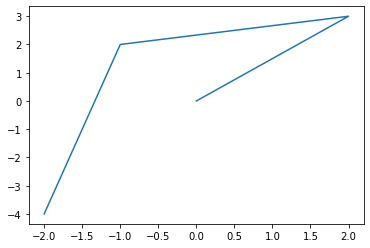
\includegraphics[width=0.5\linewidth]{figuras/pyplot01.png}
    \bicaption{Ejemplo sencillo de pyplot.} {Simple pyplot example.}
    \label{fig:pyplot-simple}
\end{figure}

\begin{paracol}{2}
    Además de las coordenadas de los puntos $(x,y)$ al método \texttt{pyplot.plot} podemos darle un tercer argumento indicando el formato (color y forma) con el que queremos que se grafiquen los puntos y opcionalmente la línea que los una. 

    Algunos de los colores y formatos admitidos están en las tablas \ref{tab:colores}, \ref{tab:puntos} y \ref{tab:lineas}. Para más información consulta la ayuda de \texttt{pyplot.plot}

    
    \begin{table}
        \centering
        \begin{tabular}{|c|c|} \hline
        \textbf{Símbolo}     &  \textbf{Color}\\
             'b'& azul \\ \hline
             'r'& rojo \\ \hline
             'g'& verde \\ \hline
             'm'& magenta\\ \hline
             'c'& cian\\ \hline
             'y'& amarillo\\ \hline
             'k'& negro\\ \hline
             'w'& blanco\\ \hline
        \end{tabular}
        \caption{Colores de los puntos}
        \label{tab:colores}
    \end{table}

    
    \begin{table}
        \centering
        \begin{tabular}{|c|c|} \hline
        \textbf{Símbolo}     &  \textbf{Formato punto}\\
             '.'& punto \\ \hline
             ','& píxel\\ \hline
             'o'& círculo \\ \hline
             's'& cuadrado\\ \hline
             '\^'& triángulo hacia abajo\\ \hline
             'v'& triángulo hacia arriba\\ \hline
             'p'& pentágono\\ \hline
             '*'& asterisco\\ \hline
        \end{tabular}
        \caption{Algunos de los marcadores de puntos}
        \label{tab:puntos}
    \end{table}

      \begin{table}
        \centering
        \begin{tabular}{|c|c|} \hline
        \textbf{Símbolo}     &  \textbf{Tipo de línea}\\
             '-'& sólida \\ \hline
             '--'& discontínua\\ \hline
             '-.'& punto-raya \\ \hline
             ':'& de puntos\\ \hline
        \end{tabular}
        \caption{Tipos de línea}
        \label{tab:lineas}
    \end{table}  
    \switchcolumn
    In addition to the coordinates of the points $(x,y)$, we can give the \texttt{pyplot.plot} method a third argument indicating the format (colour and shape) in which we want the points to be plotted and optionally the line that joins them. 

    Some of the colours and formats supported are in the tables \ref{tab:colours}, \ref{tab:dots} and \ref{tab:lines}. For more information, see the help for \texttt{pyplot.plot}.
    
    \begin{table}
        \centering
        \begin{tabular}{|c|c|} \hline
        \textbf{Symbol}     &  \textbf{Color}\\
             'b'& blue \\ \hline
             'r'& red \\ \hline
             'g'& green \\ \hline
             'm'& magenta\\ \hline
             'c'& cyan\\ \hline
             'y'& yellow\\ \hline
             'k'& black\\ \hline
             'w'& white\\ \hline
        \end{tabular}
        \caption{Point colors}
        \label{tab:colours}
    \end{table}

    
    \begin{table}
        \centering
        \begin{tabular}{|c|c|} \hline
        \textbf{Symbol}     &  \textbf{Point format}\\
             '.'& point \\ \hline
             ','& pixel\\ \hline
             'o'& circle \\ \hline
             's'& square\\ \hline
             '\^'& down triangle\\ \hline
             'v'& up triangle\\ \hline
             'p'& pentagon\\ \hline
             '*'& star\\ \hline
        \end{tabular}
        \caption{Some point markers}
        \label{tab:dots}
    \end{table}

      \begin{table}
        \centering
        \begin{tabular}{|c|c|} \hline
        \textbf{Symbol}     &  \textbf{Line type}\\
             '-'& solid \\ \hline
             '--'& dashed\\ \hline
             '-.'& dash and dot\\ \hline
             ':'& dotted\\ \hline
        \end{tabular}
        \caption{Line types}
        \label{tab:lines}
    \end{table}  
    
\end{paracol}
\section{Dibujar en 3D}
\section{Animaciones}